\subsubsection{OAuth 2.0} \label{sec:OAuth_2}

Before existence of OAuth, the access to user's protected resources was commonly delegated to a third party by sharing the user's credentials with that third party. This approach has flaws, since it is not possible for the user to fine-tune the access to their account, neither across different third parties, nor for different access levels of any given third party. 

The OAuth 1.0 was published in 2010 as to address this problem~\cite{Hammer-Lahav2010TheProtocol} and was followed in 2012 by OAuth 2.0~\cite{Hardt2012TheFramework}. OAuth 2.0 is not compatible with version 1.0 and is widely used today. In the following sections of this report we will refer to OAuth 2.0.

Using the OAuth framework, a third-party application may obtain a fine-grained access to protected resources. The third-party application requesting access to user's protected resources is known as the \textit{client}. The server controlling the protected resources has an authorisation server associated with it. The standard defines four distinct ways (called \textit{grant types}, how the client can obtain the access by communicating with the authorisation server. Before we describe these grant types, let us first draw the difference between different clients.

\paragraph{Client types} OAuth distinguishes three client types:
\begin{itemize}[noitemsep]
    \item \textit{Web-based application} is an application that runs on a web server and communicates with the user over HTML via a browser. Web-based application is considered secure, as the user and application secrets can be stored on the web server.
    \item \textit{User-agent-based application} is downloaded from the server, but afterwards runs on the user's device. This is considered less secure than web-based application, as any secrets could be potentially exposed by the user-agent (browser).
    \item \textit{Native application} is installed by the user and runs directly on user's device. It can offer good protection to secrets entered by the user during runtime, but any application secrets which are included and shipped with the application could be potentially exposed~\cite{Hardt2012TheFramework}.
\end{itemize}

\paragraph{Grant types} Four grant types are defined by the standard. Not all grant types are suitable for all client types, but other parameters, such as desired level of security or preference are also parameters for the choice of the grant type. The defined types are as follows:

\begin{itemize}[noitemsep]
    \item \textit{Authorisation Code Grant}. Using this grant type, the user is first directed from the web-based application to authenticate with the authorisation server. After user authenticates, they they are asked by the authorisation server to give consent for the client application to use the protected resources controlled by the user. Once the consent is given, the user agent receives an authorisation code from the authentication server. This authorisation code is passed to the web server via HTTP redirect method. The client running on the web server contacts the authorisation server with the authorisation code to obtain an access token. The access token is presented when the client application accesses the protected resource. This flow is illustrated in Figure~\ref{fig:oauth-code-grant}.
    \item \textit{Implicit Grant}. In this grant type, the client application is typically running in the user agent. The flow is similar to the one described above, but instead of the authorisation code, the access token is sent directly to the client application. This is simpler than the authorisation code grant, but less secure, since the access token can be captured by other applications residing on the user's device.
    \item \textit{Resource Owner Password Credentials Grant}. When using this grant type, user's credentials need to be shared directly with the client application. This is only suitable, if the client application is fully trusted by the user.
    \item \textit{Client Credentials Grant} is used when the client application requires access to own resources (as opposed to user's protected resources).
\end{itemize}

\begin{figure}[ht]
    \centering
    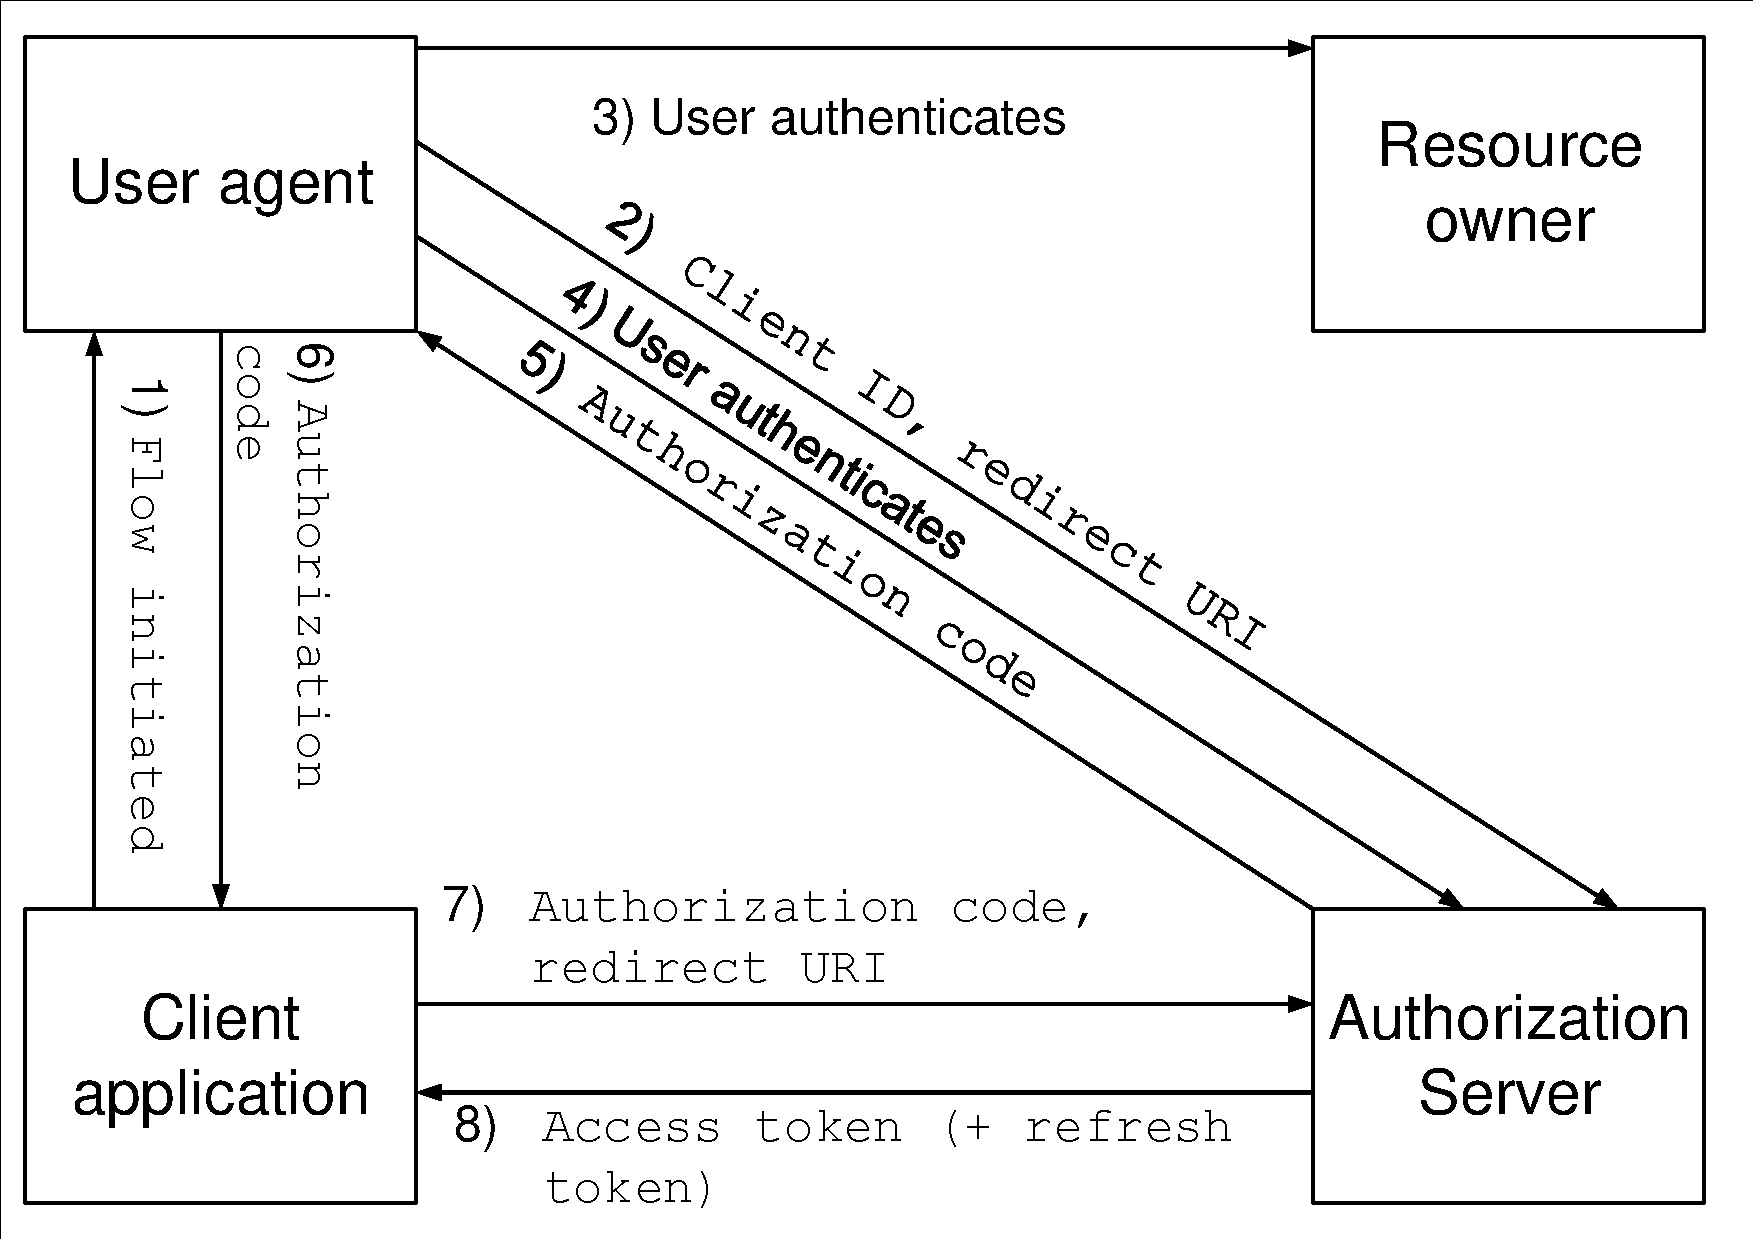
\includegraphics[width=.95\textwidth]{oauth-code-grant}
    \caption{OAuth Authorisation code grant. The user authenticates with the authorisation server and gives consent for access to their protected resources. An authorisation code is sent to the redirect URI specified in the original request. This access token is forwarded to the web server hosing the client application and exchanged for an access token at the authorisation server. From~\cite{Hardt2012TheFramework}, edited.}
    \label{fig:oauth-code-grant}
\end{figure}

\paragraph{Access token scopes}
Scope in the OAuth context typically represents a piece of functionality or data, access to which can be individually controlled. Well defined scopes allow for granular access control. The client application includes the \textit{scope} parameter in the authorisation request to inform the authorisation server, which data or functionality it wishes to access. The authorisation server may grant access to any number of the requested scopes, based on the internal policy and user's consent~\cite{Hardt2012TheFramework}.

The process outlined above is mostly concerned with authorisation of the client to access protected resources. However, it emerged as a common, albeit incorrect practice that OAuth was used to authenticate users~\cite{RicherUser2.0}, by allowing the client to only read a scope that contains the basic user data. While it is technically possible to achieve this using OAuth alone, further specifications were developed to standardise this usecase. We cover these in the following section.
% FINAL check if following section is about OpenID Connect